\documentclass{article}
\usepackage[utf8]{inputenc}
\usepackage{amsmath}
\usepackage{amssymb}
\usepackage{graphicx}
\usepackage{booktabs}
\usepackage{float}

\title{Fixed-Charge Network Flow Model for Wastewater System Design}
\author{}
\date{}

\begin{document}

\maketitle

\section{Problem Description}
This document presents a mathematical model for the wastewater system design problem. The problem involves designing a regional wastewater network that connects population centers and treatment plants with the objective of minimizing total costs.

The network consists of nodes representing population centers (where wastewater is generated) and potential locations for treatment plants. Arcs represent possible routes for main collector sewers. The goal is to determine which arcs to construct and how much flow to send through each arc, as well as where to place treatment plants.

\section{Network Structure}
The network consists of:
\begin{itemize}
    \item Nodes 1-8: Population centers with known wastewater generation (inflow)
    \item Node 9: Artificial supersink representing treated wastewater outflow
    \item Arcs: Potential sewer connections between nodes
    \item Arcs to node 9: Represent potential treatment plants
\end{itemize}

\begin{figure}[H]
    \centering
    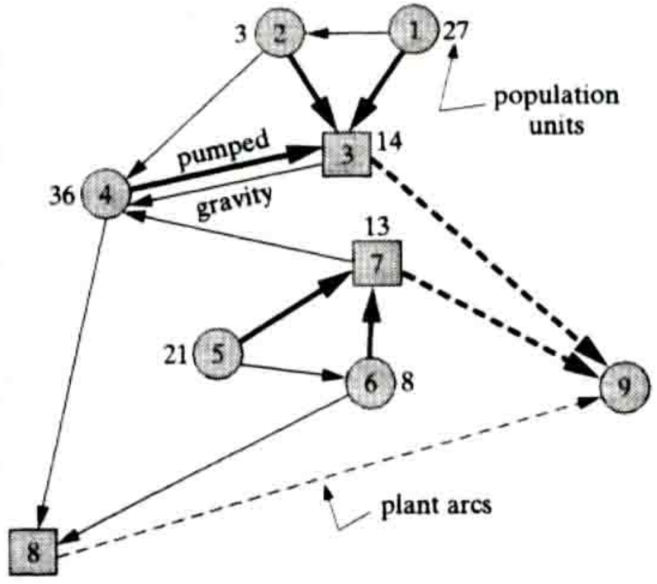
\includegraphics[width=0.8\textwidth]{fig/network_diagram.png}
    \caption{Wastewater Network Diagram}
    \label{fig:network}
\end{figure}

\section{Mathematical Model}

\subsection{Sets}
\begin{align}
    N &= \{1, 2, \ldots, 9\} \quad \text{Set of nodes} \\
    A &= \{(i,j) : \text{arc from node $i$ to node $j$ exists}\} \quad \text{Set of arcs}
\end{align}

\subsection{Parameters}
\begin{align}
    b_i &= \text{Net supply (inflow) at node $i \in N$} \\
    f_{ij} &= \text{Fixed cost for constructing arc $(i,j) \in A$} \\
    c_{ij} &= \text{Variable cost per unit flow on arc $(i,j) \in A$} \\
    u_{ij} &= \text{Capacity of arc $(i,j) \in A$}
\end{align}

For our specific instance:
\begin{itemize}
    \item $b_1 = 27, b_2 = 3, b_3 = 14, b_4 = 36, b_5 = 21, b_6 = 8, b_7 = 13, b_8 = 0, b_9 = -122$
    \item The fixed and variable costs for each arc are given in the problem statement
    \item Capacities can be derived from the network structure and population data
\end{itemize}

\subsection{Decision Variables}
\begin{align}
    x_{ij} &= \text{Flow on arc $(i,j) \in A$} \\
    y_{ij} &=
    \begin{cases}
        1 & \text{if arc $(i,j) \in A$ is constructed} \\
        0 & \text{otherwise}
    \end{cases}
\end{align}

\subsection{Objective Function}
Minimize the total cost, which includes fixed costs for constructing arcs and variable costs proportional to flow:
\begin{align}
    \min \sum_{(i,j) \in A} (f_{ij} \cdot y_{ij} + c_{ij} \cdot x_{ij})
\end{align}

\subsection{Constraints}

\subsubsection{Flow Balance Constraints}
For each node $i \in N$, the net outflow must equal the supply:
\begin{align}
    \sum_{j:(i,j) \in A} x_{ij} - \sum_{j:(j,i) \in A} x_{ji} = b_i \quad \forall i \in N
\end{align}

\subsubsection{Capacity Constraints}
The flow on each arc is limited by whether the arc is constructed and by its capacity:
\begin{align}
    x_{ij} \leq u_{ij} \cdot y_{ij} \quad \forall (i,j) \in A
\end{align}

\subsubsection{Non-negativity and Binary Constraints}
\begin{align}
    x_{ij} &\geq 0 \quad \forall (i,j) \in A \\
    y_{ij} &\in \{0,1\} \quad \forall (i,j) \in A
\end{align}

\section{Model Interpretation}
This is a fixed-charge network flow problem where:
\begin{itemize}
    \item Arcs $(i,j)$ for $i,j \in \{1,\ldots,8\}$ represent potential sewers with their associated fixed and variable costs
    \item Arcs $(i,9)$ for $i \in \{3,7,8\}$ represent potential treatment plants with their fixed and variable costs
    \item The objective is to minimize the total cost of the network while ensuring all wastewater is properly collected and treated
    \item Population centers contribute inflow to the network, which must all eventually reach node 9 (treatment)
\end{itemize}

The solution to this problem will determine:
\begin{itemize}
    \item Which sewers should be constructed (which $y_{ij} = 1$)
    \item How much flow should be sent through each constructed sewer ($x_{ij}$ values)
    \item Where treatment plants should be built (which $y_{i9} = 1$)
    \item The capacity of each treatment plant ($x_{i9}$ values)
\end{itemize}

\end{document}
